\section{Протекание процесса сухого электронно-лучевого травления при экспонировании по произвольной области}

Разработанный алгоритм моделирования процесса СЭЛТР, вообще говоря, может быть использован для моделирования результирующего профиля, получаемого при экспонировании по произвольной области. Для демонстрации возможностей алгоритма были промоделированы профили, получаемые при экспонировании электронным лучом, плотность тока в котором описывалась суммой двух (рисунок~\ref{fig:DEBER_multibeam} a)) или четырех (рисунок~\ref{fig:DEBER_multibeam}~б)) функций Гаусса. 

\begin{figure}[t!]
	\begin{minipage}{0.48\textwidth}
%		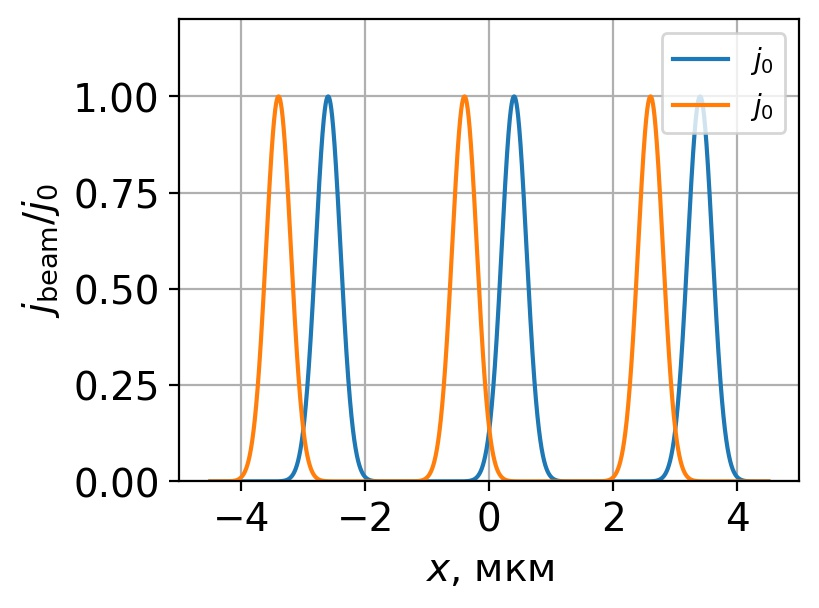
\includegraphics[width=\linewidth]{DEBER_asymmetric/pm_400_colors_200} \\
		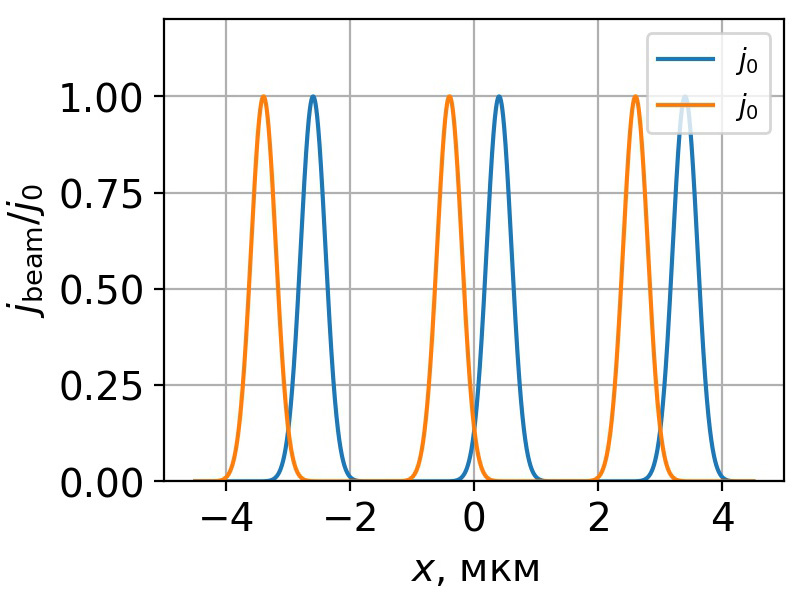
\includegraphics[width=\linewidth]{DEBER_asymmetric/pm_400_colors_200_cut} \\
		\vspace{-13em} \\ \text{\hspace{0em} a}) \\ \vspace{13em}
	\end{minipage}
	\begin{minipage}{0.48\textwidth}
		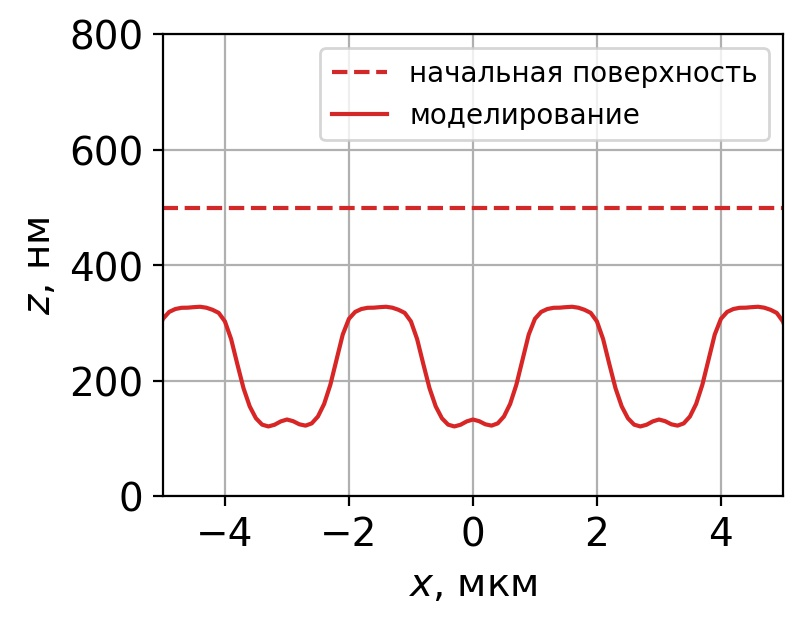
\includegraphics[width=\linewidth]{DEBER_asymmetric/pm_400_200} \\
		\vspace{-13em} \\ \text{\hspace{-0.1em} б}) \\ \vspace{13em}
	\end{minipage}
	
	\vspace{-3em}
	
	\begin{minipage}{0.48\textwidth}
		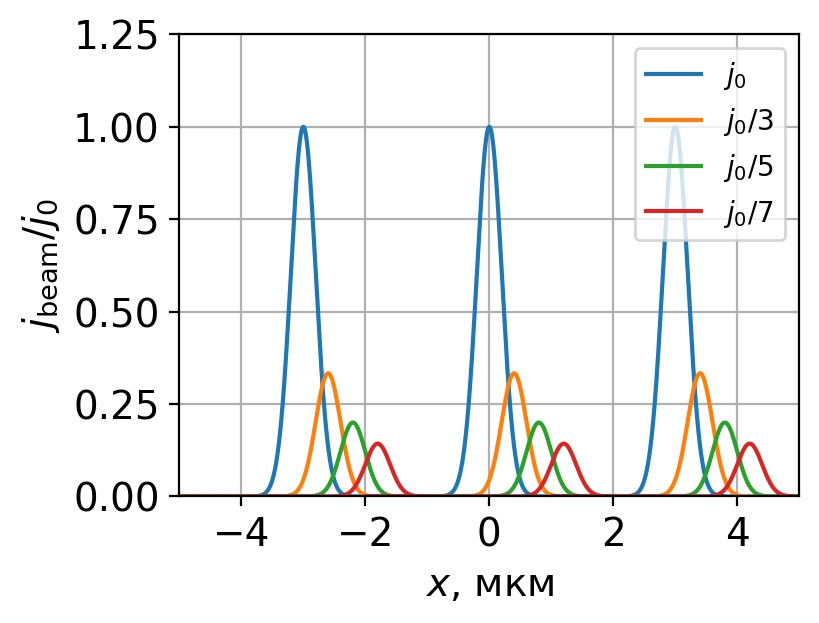
\includegraphics[width=\linewidth]{DEBER_asymmetric/asymmetric_beam_200} \\
		\vspace{-13em} \\ \text{\hspace{0em} в}) \\ \vspace{13em}
	\end{minipage}
	\begin{minipage}{0.48\textwidth}
		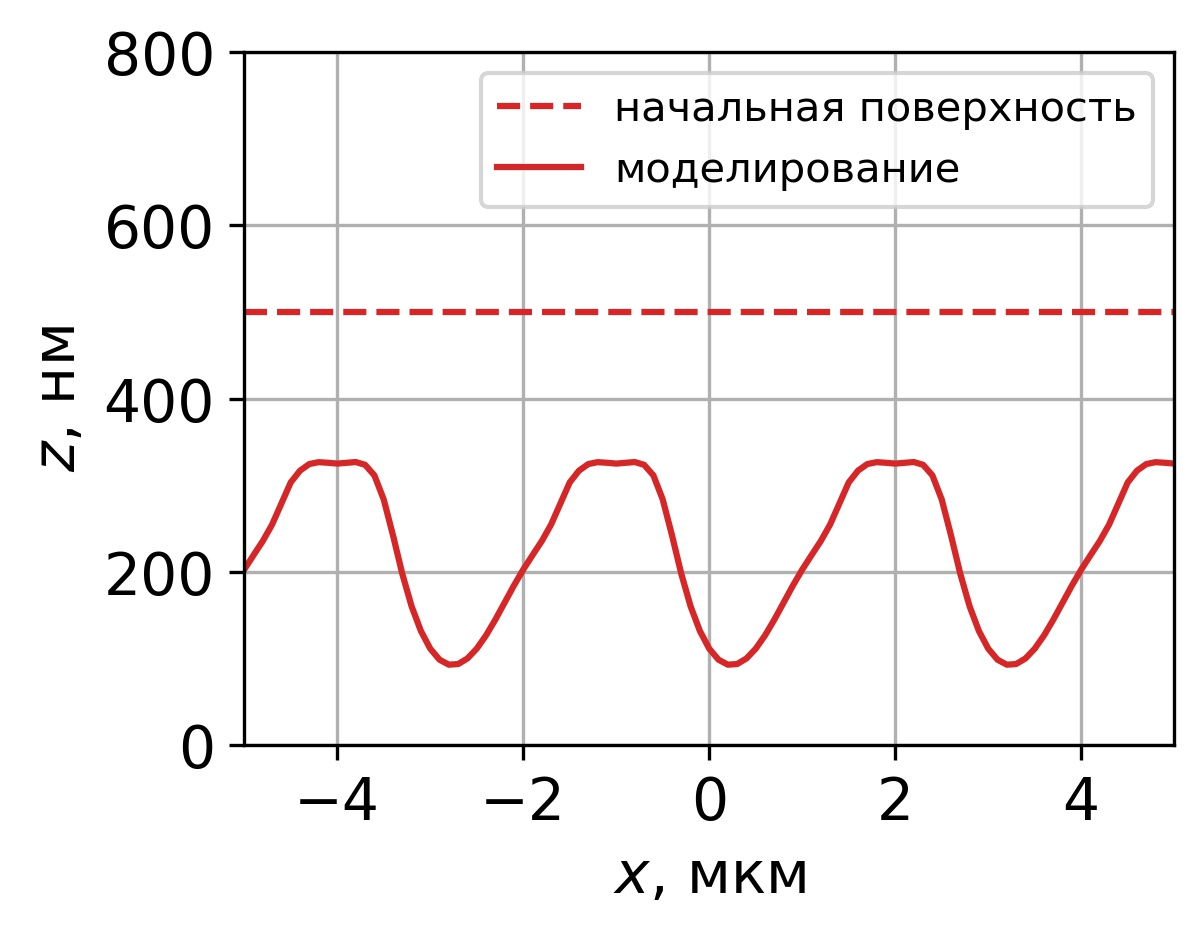
\includegraphics[width=\linewidth]{DEBER_asymmetric/asymmetric_profile_200} \\
		\vspace{-13em} \\ \text{\hspace{-0.1em} г}) \\ \vspace{13em}
	\end{minipage}
	\vspace{-3em}
	\caption{Промоделированные периодические профили с периодом 3~мкм, полученные в слое ПММА с начальной толщиной 500 нм методом СЭЛТР при экспонировании по области для двух различных распределений плотности тока в пучке. Температура резиста при экспонировании -- 150 $^\circ$C/с, время экспонирования -- 100 с, ток экспонирования -- 4.56 нА. Экспонирование резиста производится ``в кадр'' с параметрами кадра, описанными в разделе~\ref{sec:verification}. Охлаждение производится в соответствии с кривой охлаждения, приведенной на рисунке~\ref{fig:exp_cooling}.}
	\label{fig:DEBER_multibeam}
\end{figure}
